\documentclass[dvipdfmx]{jarticle}
\pagestyle{empty}
\usepackage{tikz}
\usetikzlibrary{calc,shapes,arrows.meta}
\begin{document}
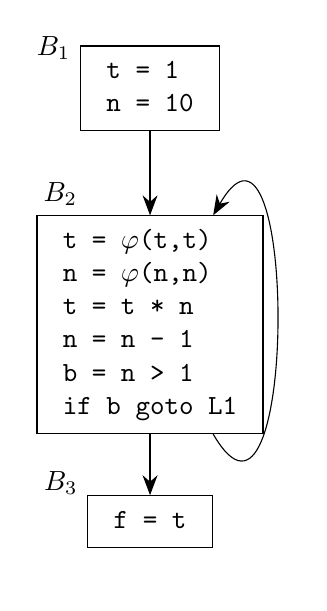
\begin{tikzpicture}
\node[draw,label={165:{$B_1$}}] (V1) at (0,0) {\begin{tabular}{l}
    \verb|t = 1|\\\verb|n = 10|\end{tabular}};
\node[draw,label={120:{$B_2$}}] (V2) at (0,-3) {\begin{tabular}{l}
    \verb|t = |$\varphi$\verb|(t,t)|\\\verb|n = |$\varphi$\verb|(n,n)|\\
    \verb|t = t * n|\\\verb|n = n - 1|\\\verb|b = n > 1|\\
    \verb|if b goto L1|\end{tabular}};
\node[draw,label={165:{$B_3$}}] (V3) at (0,-5.5) {\begin{tabular}{l}
    \verb|f = t|
\end{tabular}};
\path[-{Stealth[scale=1.5]}] (V1) edge (V2) (V2) edge (V3);
\path[-{Stealth[scale=1.5]}] (V2) [out=300,in=60,looseness=2] edge (V2);
\end{tikzpicture}
\end{document}